% Topic #3 - Evolution

%------------------------------------
% Main Settings
%------------------------------------
\documentclass[10pt]{beamer}

%--------------------------------------%
% Set font, and frame title info    %
%--------------------------------------%
\usefonttheme{serif}
\setbeamerfont{frametitle}{series=\bfseries}
\setbeamerfont{framesubtitle}{series=\bfseries}

%--------------------------------------
% "Sub-settings"
%--------------------------------------
\setbeamertemplate{navigation symbols}{}		% Get rid of navigation symbols
\setbeamertemplate{items}[default]				% Uses triangles and numbers instead of 3D balls (which I don't like)
\setbeamertemplate{itemize items}[circle]		% Use circles instead of triangles for itemized lists
\setbeamertemplate{footline}[frame number]      % Show frame #

%-------------------------------------
% Custom Commands
%-------------------------------------
\newtheorem{hypothesis}{Hypothesis}

%---For Footnotes---%
\usepackage{tikz}
\usepackage[absolute,overlay]{textpos}
\usetikzlibrary{calc,shapes.callouts,shapes.arrows,shapes,positioning}
\newenvironment{reference}[2]{%
	\begin{textblock*}{\textwidth}(#1,#2)
		\tiny\bgroup\color{gray}}{\egroup\end{textblock*}}
%------%		

%----------------------------------------%
% For making definitions in boxes        %
%----------------------------------------%
\usepackage{tcolorbox}

%--- For links ---%
\usepackage{hyperref}

%-- Packages for making nice tables --%
\usepackage{booktabs}
\usepackage{makecell}  % Required for specifying multiple rows within a table cell

%--------------------------------%
%     Custom Colours             %
%--------------------------------%
\usepackage{xcolor}
\definecolor{myblue}{rgb}{0,0.3,0.6}
\definecolor{myblue2}{rgb}{0,0.4,0.8}
\setbeamercolor{frametitle}{fg=myblue}
\setbeamercolor{framesubtitle}{fg=myblue2}
\setbeamercolor{itemize item}{fg=myblue}
\setbeamercolor{itemize subitem}{fg=myblue2}
\setbeamercolor{enumerate item}{fg=myblue}
\setbeamercolor{enumerate subitem}{fg=myblue2}


%----------------------------------%
% Creating nice blocks             %
%----------------------------------%
\setbeamercolor{block title}{bg=myblue, fg=white} %bg=background, fg=foreground
\setbeamercolor{block body}{bg=myblue!20, fg=black} %bg=background, fg=foreground
\setbeamerfont*{block title}{family=\sffamily, series=\bfseries, size=\large}
\setbeamertemplate{blocks}[rounded][shadow=true]


%------------------------%
% For making callouts    %
%------------------------%
\tikzset{
  notice/.style  = { draw, rectangle callout, callout relative pointer={#1} },
}

%------------------------------------------
%  Begin Presentations
%------------------------------------------
\begin{document}


%-----------------------%
%  Title Slide          %
%-----------------------%
\begin{frame}
	\begin{tikzpicture}[remember picture,overlay]
		\fill[color=myblue, draw=none] (current page.west) rectangle(current page.north east);
		\node at (1.5, 0.2) {\color{white}\LARGE{\textbf{Evolution}}};
	\end{tikzpicture}
\end{frame}


%----------------%
% Dobzhansky     %
%----------------%
\begin{frame}

	\begin{center}
		``\emph{Nothing in biology makes sense except in the light of evolution}''\\
		
		\vspace{0.5cm}
		
		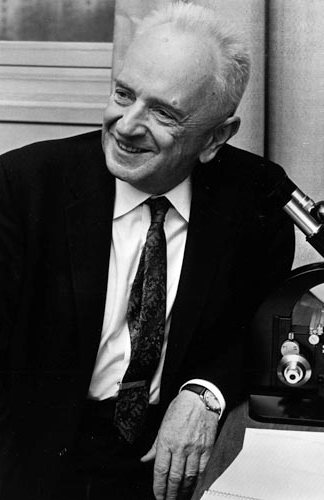
\includegraphics[width=0.25\textwidth]{figures/dobzhansky.jpg}\\
		Theodosius Dobzhansky\\
		(1900--1975)
	\end{center}
	
\end{frame}


%--------------------------%
% Evolution: Daily Life I  %
%--------------------------%
\begin{frame}[t]
\frametitle{What Is Evolution?}
\framesubtitle{In everyday life}

	\begin{center}
		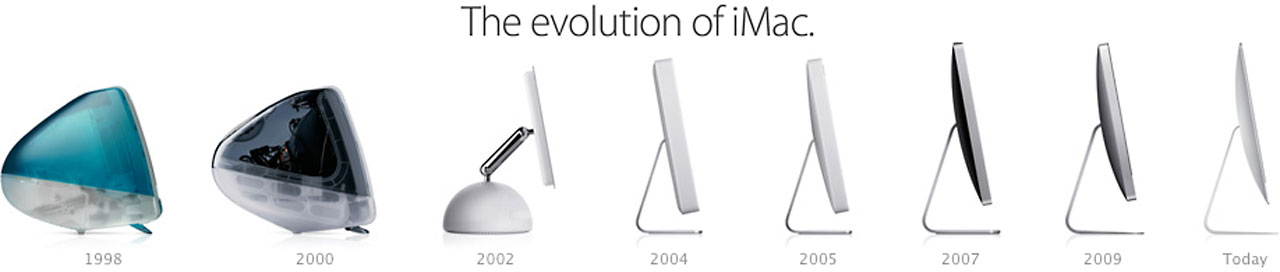
\includegraphics[width=0.7\textwidth]{figures/imac.jpg}	
	\end{center}
	
	\vspace{0.5cm}
	
	\begin{columns}
		\begin{column}{0.5\textwidth}
			\begin{center}
				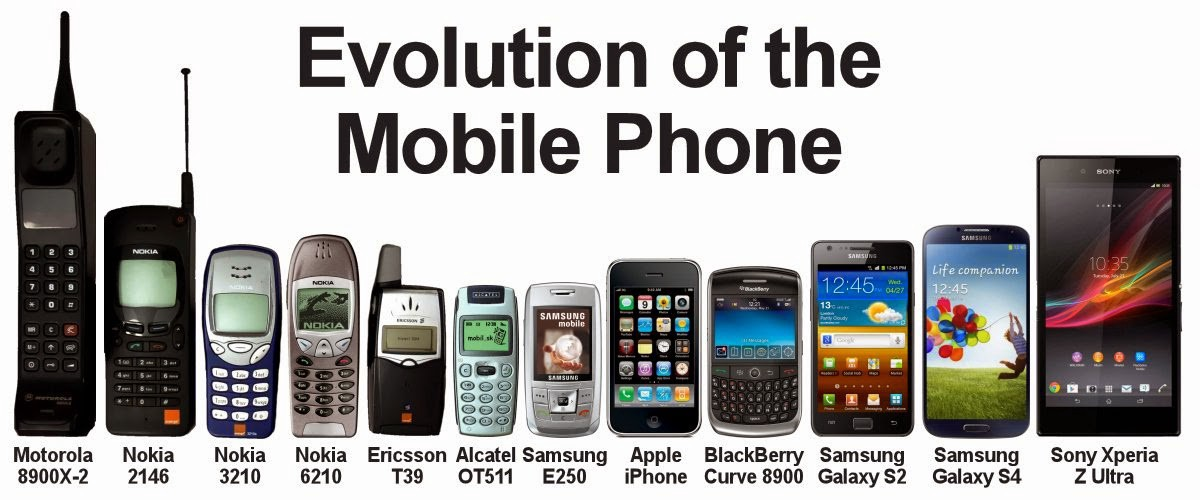
\includegraphics[width=0.9\textwidth]{figures/phone.jpg}\\	
			\end{center}
		\end{column}
		
		\begin{column}{0.5\textwidth}
			\begin{center}
				
\includegraphics[width=0.9\textwidth]{figures/hiphop.jpg}\\
			\end{center}
		\end{column}	
	\end{columns}

\end{frame}


%--------------------------%
% Evolution: Daily Life I  %
%--------------------------%
\begin{frame}[t]
\frametitle{What Is Evolution?}
\framesubtitle{In everyday life}

	\begin{center}
		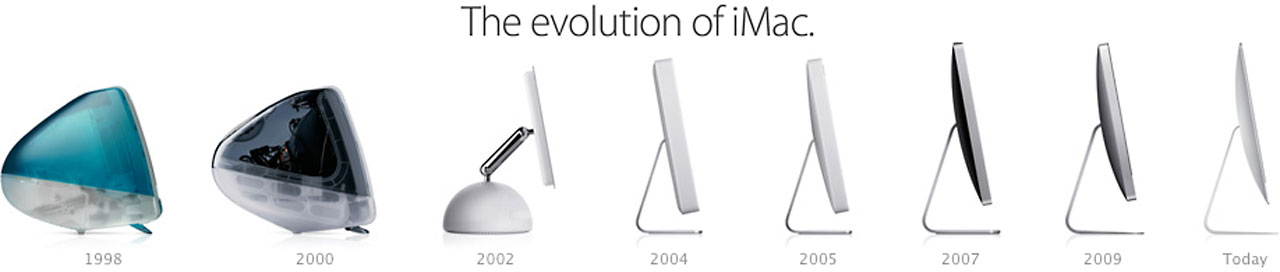
\includegraphics[width=0.7\textwidth]{figures/imac.jpg}\\
	\end{center}

	\vspace{0.25cm}
		
	\begin{center}
		\textcolor{myblue}{``Change over time''}
	\end{center}
\end{frame}


%---------------------------%
% Evolution: Daily Life II  %
%---------------------------%
\begin{frame}[t]
\frametitle{What Is Evolution?}
\framesubtitle{In everyday life}
\vspace{0.5cm}

	\begin{center}
		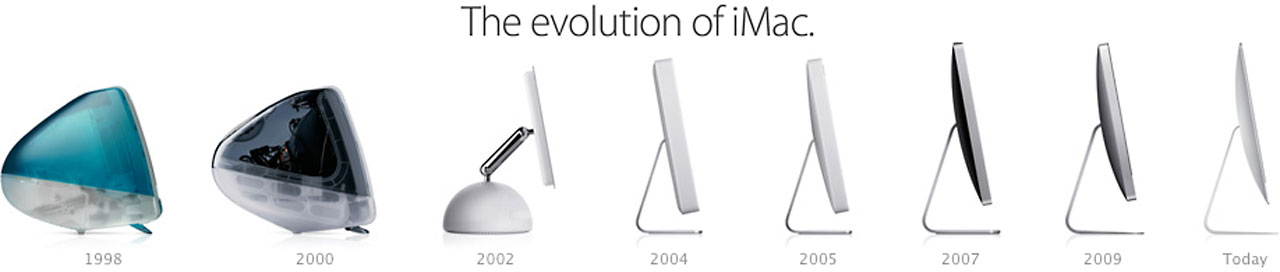
\includegraphics[width=0.9\textwidth]{figures/imac.jpg}
	\end{center}

\textcolor{myblue}{Did each individual computer change?	}

	\pause
	
	\vspace{0.5cm}
	
	No, the \emph{information} on how to build computers is what changed
\end{frame}


%--------------------------%
% Evolution: Biology I     %
%--------------------------%
\begin{frame}[t]
\frametitle{What Is Evolution?}
\framesubtitle{In biology}
\vspace{0.5cm}

	Similar to in daily life\\
	
	\vspace{0.25cm}
	
	\begin{columns}[t]
		\begin{column}{0.6\textwidth}
			\begin{center}
				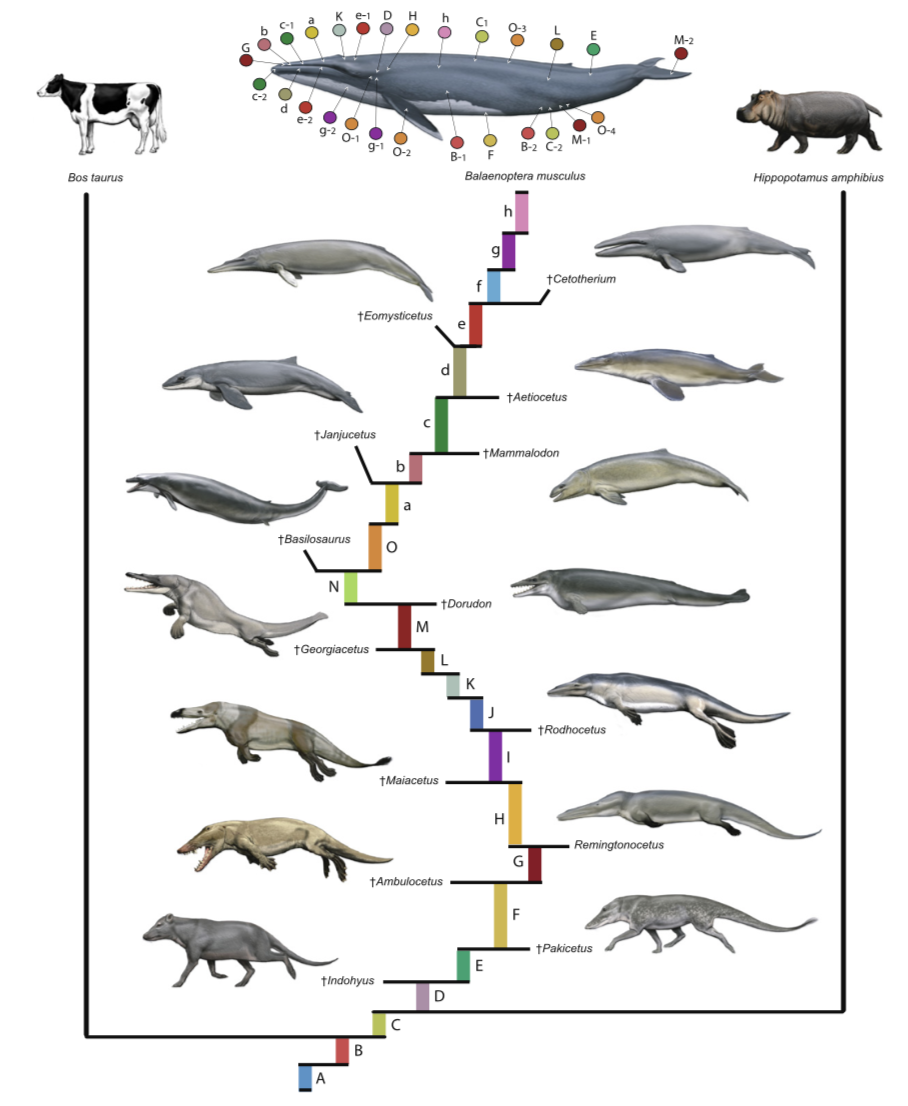
\includegraphics[width=0.7\textwidth]{figures/evolution.png}
			\end{center}
		\end{column}	
		
		\begin{column}{0.4\textwidth}
			\begin{center}
				\textcolor{myblue}{What represents the instructions/information for how to build biological organisms?}
			\end{center}
		\end{column}
	\end{columns}
\end{frame}


%--------------------------%
% Evolution: Biology II    %
%--------------------------%
\begin{frame}[t]
\frametitle{What Is Evolution?}
\framesubtitle{In biology}
\vspace{0.5cm}

	Similar to in daily life\\
	
	\vspace{0.25cm}
	
	\begin{columns}[t]
		\begin{column}{0.6\textwidth}
			\begin{center}
				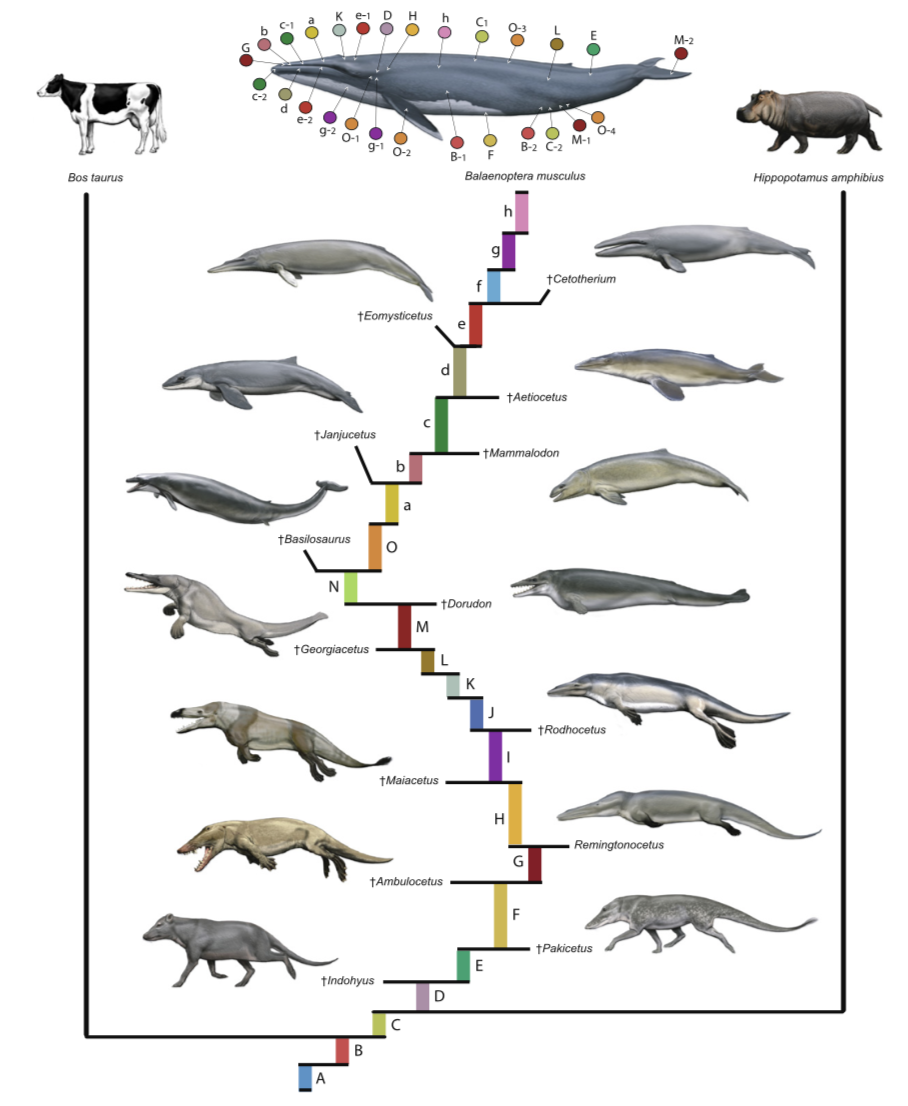
\includegraphics[width=0.7\textwidth]{figures/evolution.png}
			\end{center}
		\end{column}	
		
		\begin{column}{0.4\textwidth}
			\begin{center}
				\textcolor{myblue}{What represents the instructions/information for how to build biological organisms?}\\
				\vspace{0.5cm}
				\textcolor{red}{\textbf{DNA}}
			\end{center}
		\end{column}
	\end{columns}
\end{frame}


%--------------------------%
% Evolution: Biology III   %
%--------------------------%
\begin{frame}[t]
\frametitle{What Is Evolution?}
\framesubtitle{In biology}
\vspace{0.5cm}

	``\textcolor{myblue}{\emph{Heritable} change over time}''

	\vspace{0.5cm}

	``Descent with modification''

	\vspace{0.5cm}
	
	\begin{center}
		\textbf{\emph{Heritable} traits are what are important for evolution}
	\end{center}
	
\end{frame}


%--------------------------%
% Evolution: Biology IV    %
%--------------------------%
\begin{frame}[t]
\frametitle{What Is Evolution?}
\framesubtitle{In biology}

	\begin{center}
		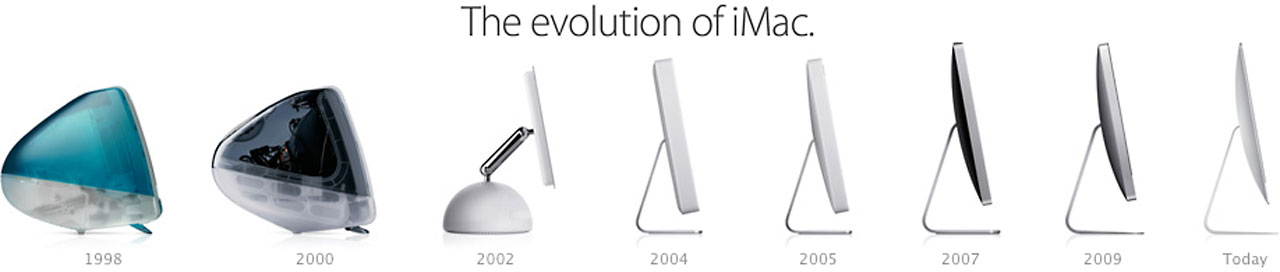
\includegraphics[width=0.5\textwidth]{figures/imac.jpg}\\
		\vspace{0.5cm}
		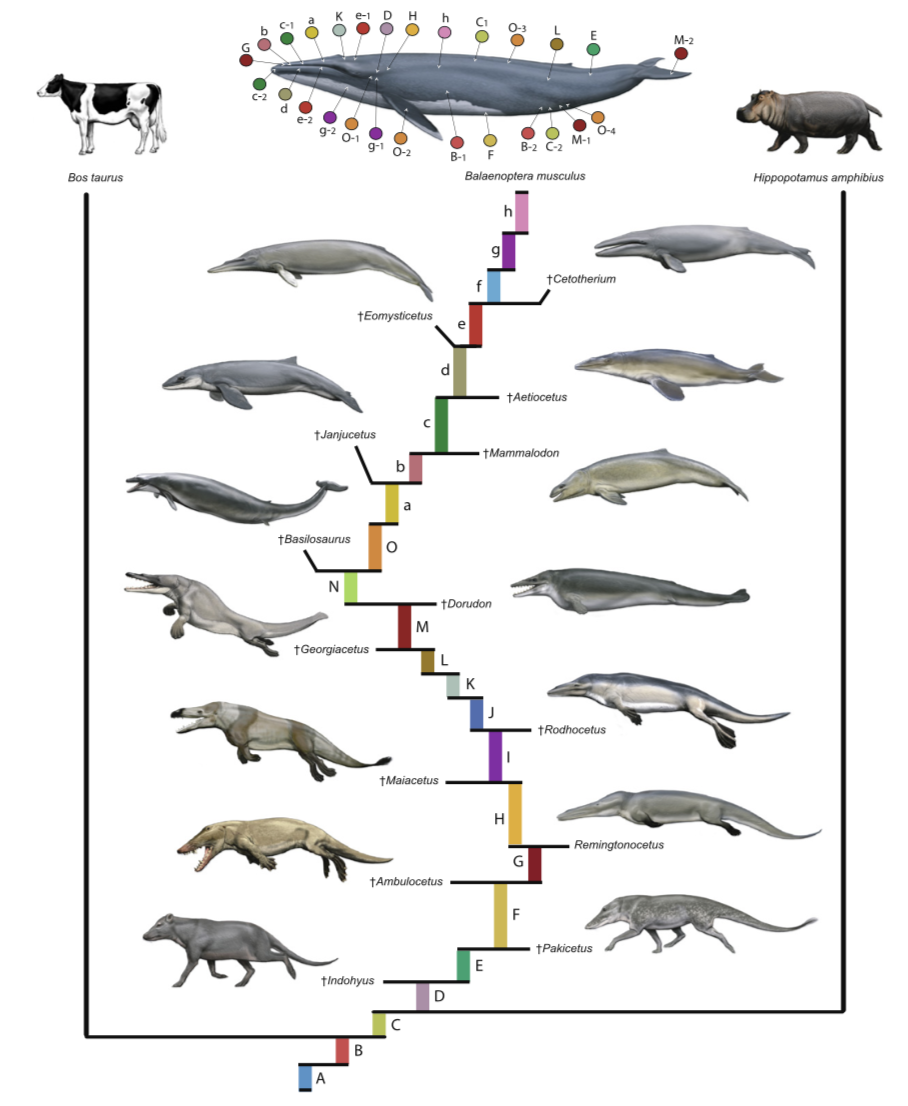
\includegraphics[width=0.45\textwidth]{figures/evolution.png}
	\end{center}
\end{frame}


%-----------------------%
% Acquired Characters I %
%-----------------------%
\begin{frame}[t]
\frametitle{What Is Evolution?}
\vspace{0.5cm}

	Organisms do not evolve within their lifetime (no heredity)\\
		\begin{itemize}
			\item ``My thoughts on the relative merits of communism \emph{vs} democracy have evolved as I've aged.''
			\smallskip
			\item Not biological evolution, but more in the day-to-day usage\\
		\end{itemize}
	
	\vspace{0.5cm}
	Traits that we accumulate over our lifetimes are called \textcolor{myblue}{\emph{acquired}} traits
		\smallskip
		\begin{itemize}
			\item We do not pass on acquired traits to our offspring (for the most part)
		\end{itemize}	
\end{frame}


%-------------------------%
% Acquired Characters II  %
%-------------------------%
\begin{frame}[t]

	\begin{tikzpicture}[overlay]
		\node at (1.0, -2.0) (wimpy) {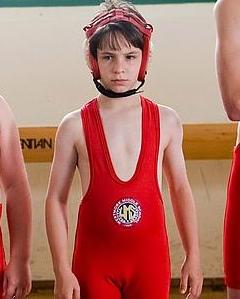
\includegraphics[width=0.220\textwidth]{figures/wimpy.jpg}};
		\node at (4.0, -2.0) (strong) {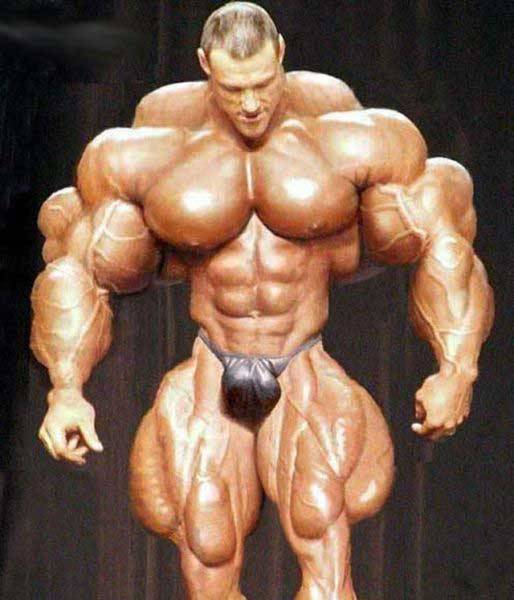
\includegraphics[width=0.225\textwidth]{figures/strong.jpg}};
		\draw[->, >=latex, thick] (wimpy)--(strong);
	\end{tikzpicture}
	
	\pause
	
	\begin{tikzpicture}[overlay]
		\draw[->, >=latex, thick] (2.5, -3.25) -- (2.5, -5.5);
		\node at (2.5, -6.0) (sperm) {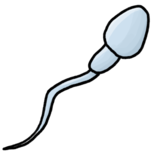
\includegraphics[width=0.15\textwidth]{figures/sperm.png}};
		\node at (2.5, -4.25) (no) {
\includegraphics[width=0.15\textwidth]{figures/no.png}};
	\end{tikzpicture}
\end{frame}


%-------------------------%
% Acquired Characters III %
%-------------------------%
\begin{frame}[t]

	\begin{tikzpicture}
		\node at (1.0, -2.0) (wimpy) {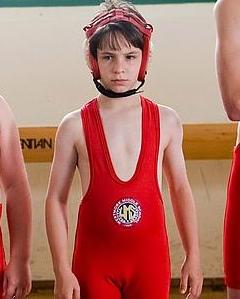
\includegraphics[width=0.220\textwidth]{figures/wimpy.jpg}};
		\node at (4.0, -2.0) (strong) {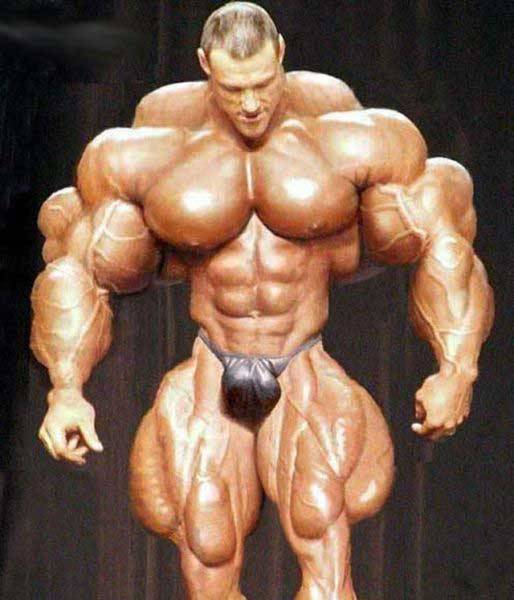
\includegraphics[width=0.225\textwidth]{figures/strong.jpg}};
		\draw[->, >=latex, thick] (wimpy)--(strong);
		\draw[->, >=latex, thick] (2.5, -3.5) -- (2.5, -6.25);
		\node at (2.5, -7.0) (sperm) {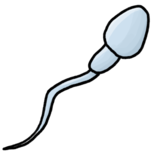
\includegraphics[width=0.15\textwidth]{figures/sperm.png}};
		\node at (2.5, -5.0) (no) {
\includegraphics[width=0.15\textwidth]{figures/no.png}};
		
		\node at (7.0, -2.0) (paris) {
\includegraphics[width=0.15\textwidth]{figures/paris.jpg}};
		\node at (10.0, -2.0) (doctor) {
\includegraphics[width=0.175\textwidth]{figures/doctor.png}};
		\draw[->, >=latex, thick] (paris)--(doctor);
		\draw[->, >=latex, thick] (8.5, -3.5) -- (8.5, -6.25);
		\node at (8.5, -7.0) (egg) {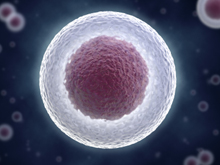
\includegraphics[width=0.15\textwidth]{figures/egg.jpg}};
		\node at (8.5, -5.0) (no) {
\includegraphics[width=0.15\textwidth]{figures/no.png}};
	\end{tikzpicture}
\end{frame}


%-------------------------%
% Acquired Characters IV  %
%-------------------------%
\begin{frame}
	\begin{center}
		\textbf{\emph{Heritable} traits are what are important for evolution}
	\end{center}
\end{frame}

	
%-------------------------%
% What Causes Change      %
%-------------------------%
\begin{frame}[t]
\frametitle{What Causes DNA to Change Over Time?}
\vspace{0.5cm}

	A two-stage process:
	\smallskip
	
		\begin{enumerate}
			\item The introduction of variation
			\smallskip
			\item Differential ``success'' of individuals with different traits
		\end{enumerate}
\end{frame}		


%-------------------------%
% What Causes Change II   %
%-------------------------%
\begin{frame}[t]
\frametitle{What Causes DNA to Change Over Time?}
\vspace{0.5cm}

	A two-stage process:
	\smallskip
	
		\begin{enumerate}
			\item The introduction of variation
			\smallskip
			\item \textcolor{gray}{Differential ``success'' of individuals with different traits}
		\end{enumerate}
\end{frame}		


%-------------------------%
% Sources of Variation I  %
%-------------------------%
\begin{frame}[t]
\frametitle{What Causes DNA to Change Over Time?}
\framesubtitle{1. Sources of variation}
\vspace{0.5cm}

	Are three main sources of variation:
	\medskip
		\begin{enumerate}
			\item[a.] Mutations
			\medskip
			\item[b.] Recombination
			\medskip
			\item[c.] Sexual reproduction (for some species)
		\end{enumerate}

\end{frame}


%-------------------------%
% Sources of Variation II %
%-------------------------%
\begin{frame}[t]
\frametitle{What Causes DNA to Change Over Time?}
\framesubtitle{1. Sources of variation}
\vspace{0.5cm}

	\textbf{\textcolor{myblue}{a.} Mutations}\\
		\medskip
		\begin{itemize}
			\item DNA gets replicated prior to cell division
			\medskip
			\item During replication, errors randomly occur along the DNA sequence
				\smallskip
				\begin{itemize}
					\item Many neutral or nearly so (95\% of human genome is non-coding)
					\smallskip
					\item Many detrimental
					\smallskip
					\item Few may be beneficial\\
				\end{itemize}
			\medskip
			\item Only those along the \textcolor{myblue}{germ line} are important in evolution 	
		\end{itemize}
\end{frame}


%----------------------------------%
% Somatic vs Germ-line Mutations 1 %
%----------------------------------%
\begin{frame}[t]
\frametitle{Somatic \emph{vs} Germ-line Mutations}
\vspace{0.25cm}

	Can divide cell lines into two types:\\
		\smallskip
	
		\begin{columns}
			\begin{column}{0.5\textwidth}
				\begin{enumerate}
					\item \textbf{\textcolor{red}{Germ-line}} cells: cells that give rise to your gametes (eggs \& sperm)
					\smallskip
					\item \textbf{\textcolor{myblue}{Somatic}} cells: the rest of the cells in your body (i.e., cells that don't give rise to gametes)
				\end{enumerate}
			\end{column}
			
			\begin{column}{0.5\textwidth}
				\centerline{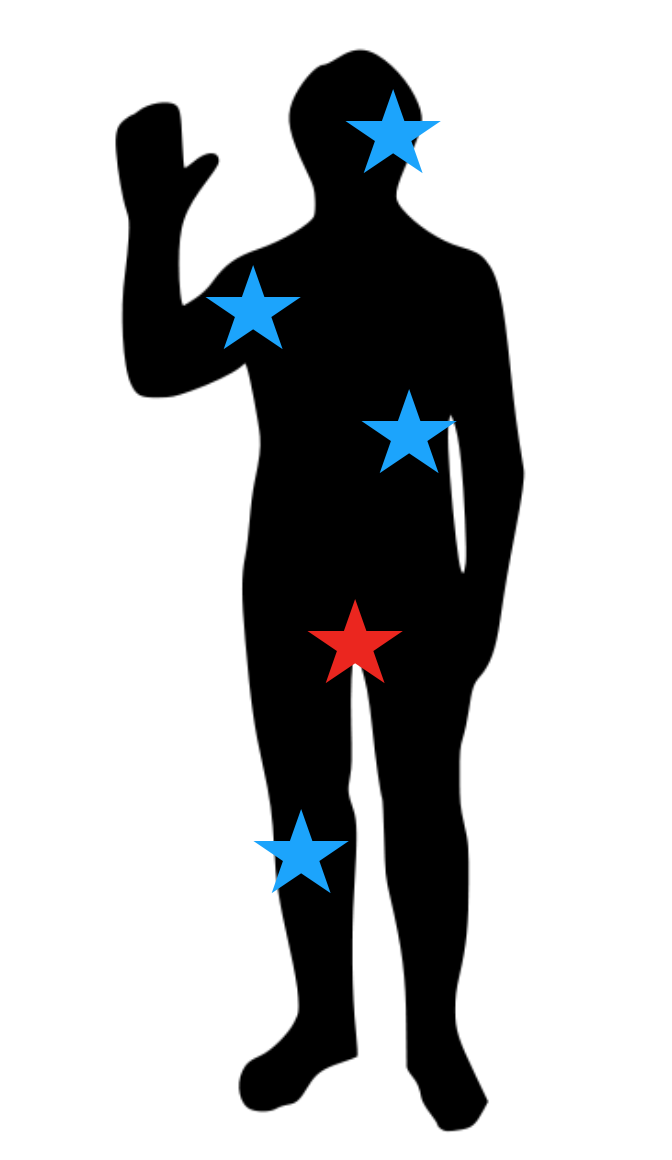
\includegraphics[width=0.5\textwidth]{figures/mutation-types.png}}
			\end{column}
		\end{columns}	
	
	\vspace{0.5cm}
	
	\begin{center}
		\textcolor{myblue}{\emph{Mutations in each of these cells lines have vastly different implications!}}
	\end{center}
\end{frame}


%----------------------------------%
% Somatic vs Germ-line Mutations 2 %
%----------------------------------%
\begin{frame}[t]
\frametitle{Somatic \emph{vs} Germ-line Mutations}
\vspace{0.25cm}

	Mutations in \textcolor{myblue}{somatic cells} \textbf{are not} passed on to offspring \\
		\smallskip
		\begin{itemize}
			\item Directly impact just your body
			\smallskip
			\item Not too important for evolution (except when they kill you before you reproduce)
		\end{itemize}
	
	\vspace{0.25cm}
	
	\begin{columns}
		\begin{column}{0.5\textwidth}
			\centerline{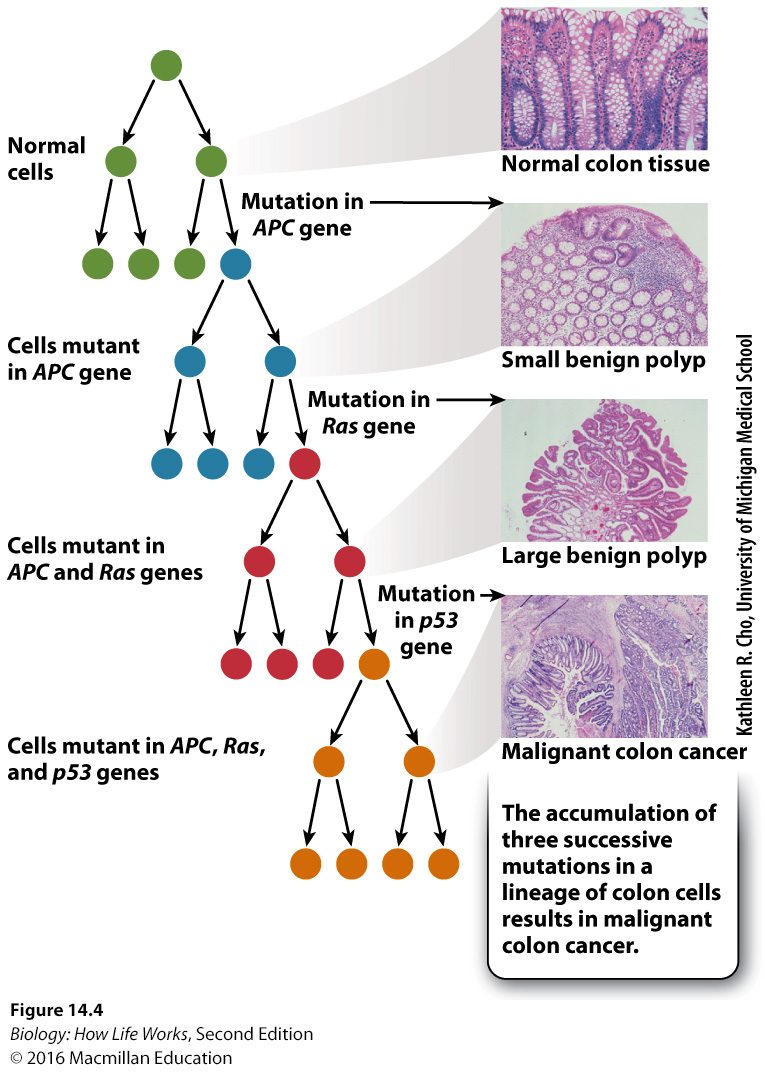
\includegraphics[width=0.7\textwidth]{figures/figure_14_04.jpg}}
		\end{column}
		
		\begin{column}{0.5\textwidth}
			\centerline{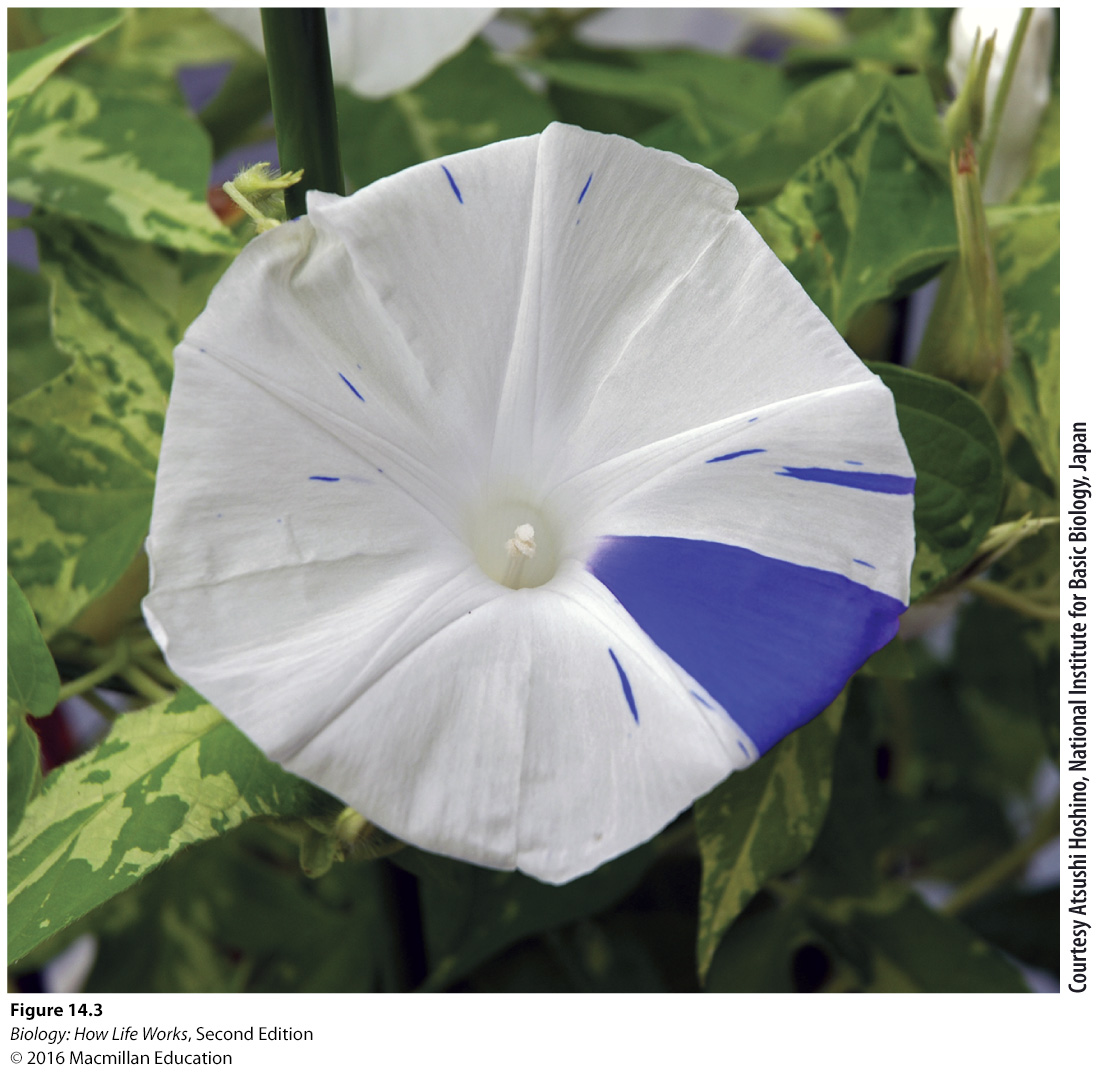
\includegraphics[width=0.7\textwidth]{figures/figure_14_03.jpg}}
		\end{column}
	\end{columns}	
\end{frame}


%----------------------------------%
% Somatic vs Germ-line Mutations 3 %
%----------------------------------%
\begin{frame}[t]
\frametitle{Somatic \emph{vs} Germ-line Mutations}
\vspace{0.25cm}
		
	Mutations in \textcolor{myblue}{germ-line cells} \textbf{are} passed on to offspring \\
		\smallskip
		\begin{itemize}
			\item Main types of mutation important for evolution
		\end{itemize}
	
	\vspace{0.25cm}
	
	\begin{center}
		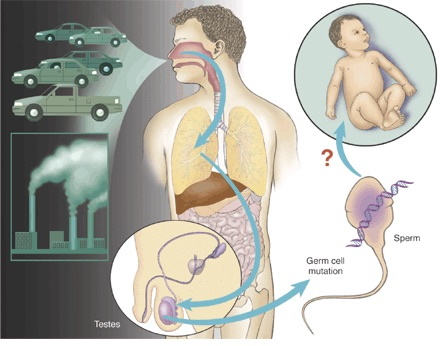
\includegraphics[width=0.55\textwidth]{figures/pollution.jpg}
	\end{center}
\end{frame}


%--------------------------%
% Sources of Variation III %
%--------------------------%
\begin{frame}[t]
\frametitle{What Causes DNA to Change Over Time?}
\framesubtitle{1. Sources of variation}
\vspace{0.5cm}

	Are three main sources of variation:
	\medskip
		\begin{enumerate}
			\item[a.] \textcolor{gray}{Mutations}
			\medskip
			\item[b.] Recombination
			\medskip
			\item[c.] \textcolor{gray}{Sexual reproduction (for some species)}
		\end{enumerate}
\end{frame}


%-------------------------%
% Sources of Variation IV %
%-------------------------%
\begin{frame}[t]
\frametitle{What Causes DNA to Change Over Time?}
\framesubtitle{1. Sources of variation}
\vspace{0.5cm}

	\textbf{\textcolor{myblue}{b.} Recombination/Crossing Over}\\
		\medskip
		\begin{itemize}
			\item The exchange of genetic material between homologous chromosomes during meiosis (\textcolor{myblue}{\emph{in-depth later}})
			\medskip
			\item Changes the \emph{arrangement} of genetic material, but not it's \emph{content} 	
		\end{itemize}
		
		\vspace{0.25cm}
		
		\begin{center}
			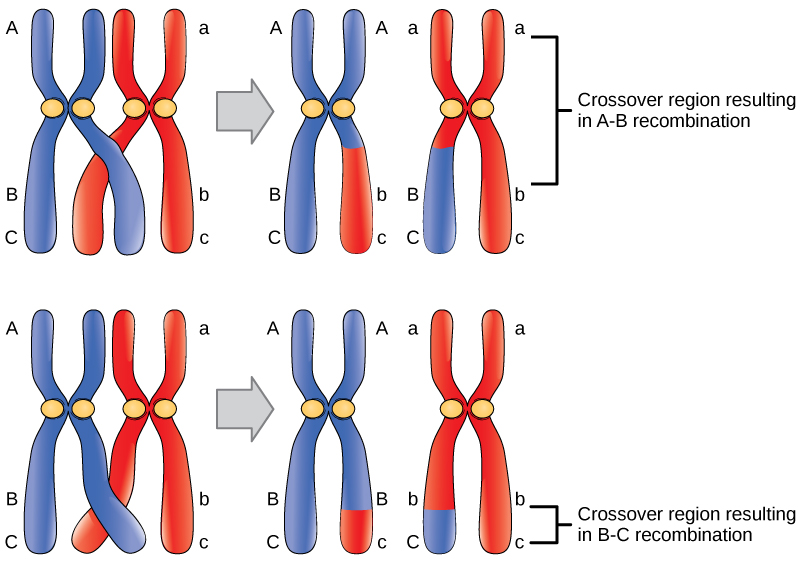
\includegraphics[width=0.5\textwidth]{figures/crossing_over.jpg}
		\end{center}
\end{frame}


%--------------------------%
% Sources of Variation V   %
%--------------------------%
\begin{frame}[t]
\frametitle{What Causes DNA to Change Over Time?}
\framesubtitle{1. Sources of variation}
\vspace{0.5cm}

	Are three main sources of variation:
	\medskip
		\begin{enumerate}
			\item[a.] \textcolor{gray}{Mutations}
			\medskip
			\item[b.] \textcolor{gray}{Recombination}
			\medskip
			\item[c.] Sexual reproduction (for some species)
		\end{enumerate}
\end{frame}


%-------------------------%
% Sources of Variation VI %
%-------------------------%
\begin{frame}[t]
\frametitle{What Causes DNA to Change Over Time?}
\framesubtitle{1. Sources of variation}
\vspace{0.5cm}

	\textbf{\textcolor{myblue}{c.} Sexual reproduction}\\
		\medskip
		\begin{itemize}
			\item Results in new combinations of DNA sequences	
		\end{itemize}
		
		\vspace{0.5cm}
		
		\begin{center}
			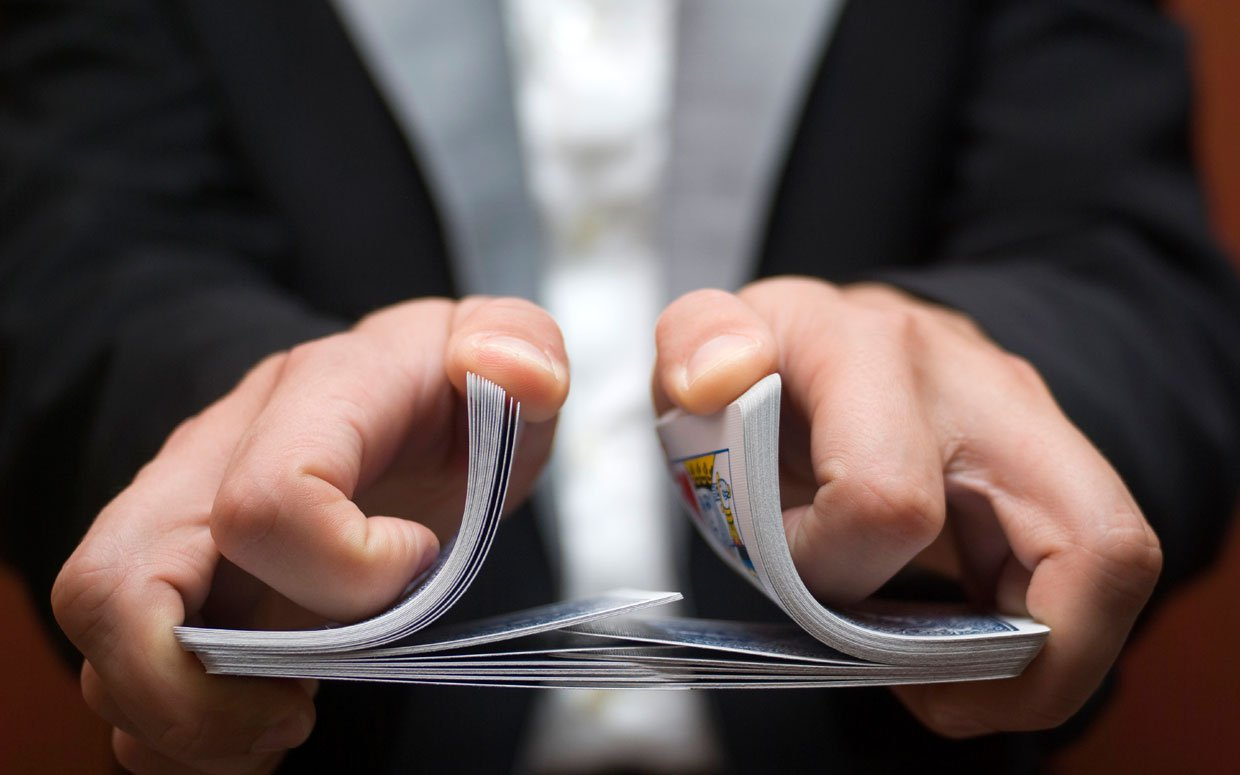
\includegraphics[width=0.6\textwidth]{figures/cards.jpg}
		\end{center}
\end{frame}


%--------------------------%
% Sources of Variation VII %
%--------------------------%
\begin{frame}[t]
\frametitle{What Causes DNA to Change Over Time?}
\framesubtitle{1. Sources of variation}
\vspace{0.5cm}

	\begin{tikzpicture}[overlay]
		\node[draw=gray, fill=gray!30, rounded corners, minimum width=2.5cm, minimum height = 1.5cm] at (5.1, -0.8) (node1) {};
	
		\draw[draw=blue, fill=blue!30] (4.3,-1.1) circle (2.5pt);
		\draw[draw=blue, fill=blue!30] (4.2,-0.9) circle (2.5pt);
		\draw[draw=blue, fill=blue!30] (6.0,-0.8) circle (2.5pt);
		\draw[draw=blue, fill=blue!30] (5.4,-0.5) circle (2.5pt);
		\draw[draw=blue, fill=blue!30] (4.8,-0.5) circle (2.5pt);
		\draw[draw=blue, fill=blue!30] (5.8,-1.1) circle (2.5pt);
		\draw[draw=blue, fill=blue!30] (5.6,-1.1) circle (2.5pt);
		\draw[draw=blue, fill=blue!30] (4.4,-0.6) circle (2.5pt);
		\draw[draw=blue, fill=blue!30] (4.5,-1.0) circle (2.5pt);
		\draw[draw=blue, fill=blue!30] (5.6,-0.6) circle (2.5pt);
		\draw[draw=blue, fill=blue!30] (4.9,-0.7) circle (2.5pt);
		\draw[draw=blue, fill=blue!30] (6.0,-1.2) circle (2.5pt);
		\draw[draw=blue, fill=blue!30] (5.0,-1.1) circle (2.5pt);
		\draw[draw=blue, fill=blue!30] (4.2,-0.5) circle (2.5pt);
		\draw[draw=blue, fill=blue!30] (6.0,-0.5) circle (2.5pt);
		
		\node at (2, -1.8) (mutations) {\footnotesize{mutations}};
		\node at (2, -2.5) (recombination) {\footnotesize{recombination}};
		\node at (2, -3.2) (sex) {\footnotesize{sexual reproduction}};
		\node at (5.1, -2.73) (centre) {};
		\draw[->, >=latex] (mutations) -- (centre);
		\draw[->, >=latex] (recombination) -- (centre);
		\draw[->, >=latex] (sex) -- (centre);
		
		\node[draw=gray, fill=gray!30, rounded corners, minimum width=2.5cm, minimum height = 1.5cm] at (5.1, -4.65) (node2) {};
		\draw[->, >=latex, thick] (node1) -- (node2);
	
		\draw[draw=blue, fill=blue!30] (4.3,-4.1) circle (2.5pt);
		\draw[draw=red, fill=red!30] (4.2,-4.9) circle (2.5pt);
		\draw[draw=blue, fill=blue!30] (6.0,-4.8) circle (2.5pt);
		\draw[draw=blue, fill=blue!30] (5.4,-4.5) circle (2.5pt);
		\draw[draw=orange, fill=orange!30] (4.8,-4.5) circle (2.5pt);
		\draw[draw=olive, fill=olive!30] (5.8,-5.1) circle (2.5pt);
		\draw[draw=olive, fill=olive!30] (5.6,-5.1) circle (2.5pt);
		\draw[draw=purple, fill=purple!30] (4.4,-4.6) circle (2.5pt);
		\draw[draw=blue, fill=blue!30] (4.5,-5.0) circle (2.5pt);
		\draw[draw=red, fill=red!30] (5.6,-4.6) circle (2.5pt);
		\draw[draw=blue, fill=blue!30] (4.9,-4.7) circle (2.5pt);
		\draw[draw=red, fill=red!30] (6.0,-5.2) circle (2.5pt);
		\draw[draw=blue, fill=blue!30] (5.0,-5.1) circle (2.5pt);
		\draw[draw=olive, fill=olive!30] (4.2,-4.5) circle (2.5pt);
		\draw[draw=olive, fill=olive!30] (6.0,-4.5) circle (2.5pt);	
	\end{tikzpicture}
\end{frame}


%-------------------------%
% What Causes Change III  %
%-------------------------%
\begin{frame}[t]
\frametitle{What Causes DNA to Change Over Time?}
\vspace{0.5cm}

	A two-stage process:
	\smallskip
	
		\begin{enumerate}
			\item \textcolor{gray}{The introduction of variation}
			\smallskip
			\item Differential ``success'' of individuals with different traits
		\end{enumerate}
\end{frame}		


%--------------------------%
% Differential Success I   %
%--------------------------%
\begin{frame}[t]
\frametitle{What Causes DNA to Change Over Time?}
\framesubtitle{2. Differential ``success'' of individuals with different traits}	
\vspace{0.5cm}

	\begin{columns}[t]
		\begin{column}{0.5\textwidth}
			Individuals with traits allowing them to better survive and reproduce will have more offspring\\
			\vspace{1cm}
			Those traits will be more common in the next generation\\
			\vspace{1cm}
			``\textbf{Natural selection}''\\
			\emph{Nature is ``selecting'' which types are most successful}
		\end{column}
		
		\begin{column}{0.5\textwidth}
			\begin{tikzpicture}[overlay]
				\node[draw=gray, fill=gray!30, rounded corners, minimum width=2.5cm, minimum height = 1.5cm] at (2.1, -0.65) (node1) {};
				\draw[draw=blue, fill=blue!30] (1.3,-0.1) circle (2.5pt);
				\draw[draw=red, fill=red!30] (1.2,-0.9) circle (2.5pt);
				\draw[draw=blue, fill=blue!30] (3.0,-0.8) circle (2.5pt);
				\draw[draw=blue, fill=blue!30] (2.4,-0.5) circle (2.5pt);
				\draw[draw=orange, fill=orange!30] (1.8,-0.5) circle (2.5pt);
				\draw[draw=olive, fill=olive!30] (2.8,-1.1) circle (2.5pt);
				\draw[draw=olive, fill=olive!30] (2.6,-1.1) circle (2.5pt);
				\draw[draw=purple, fill=purple!30] (1.4,-0.6) circle (2.5pt);
				\draw[draw=blue, fill=blue!30] (1.5,-1.0) circle (2.5pt);
				\draw[draw=red, fill=red!30] (2.6,-0.6) circle (2.5pt);
				\draw[draw=blue, fill=blue!30] (1.9,-0.7) circle (2.5pt);
				\draw[draw=red, fill=red!30] (3.0,-1.2) circle (2.5pt);
				\draw[draw=blue, fill=blue!30] (2.0,-1.1) circle (2.5pt);
				\draw[draw=olive, fill=olive!30] (1.2,-0.5) circle (2.5pt);
				\draw[draw=olive, fill=olive!30] (3.0,-0.5) circle (2.5pt);
				
				\node[draw=gray, fill=gray!30, rounded corners, minimum width=2.5cm, minimum height = 1.5cm] at (2.1, -4.5) (node2) {};
				\draw[->, >=latex, thick] (node1) -- (node2);
				
				\draw[draw=red, fill=red!30] (1.4,-3.95) circle (2.5pt);
				\draw[draw=red, fill=red!30] (1.1,-4.75) circle (2.5pt);
				\draw[draw=orange, fill=orange!30] (3.2,-4.65) circle (2.5pt);
				\draw[draw=blue, fill=blue!30] (2.2,-4.35) circle (2.5pt);
				\draw[draw=orange, fill=orange!30] (1.95,-4.35) circle (2.5pt);
				\draw[draw=red, fill=red!30] (2.7,-4.95) circle (2.5pt);
				\draw[draw=red, fill=red!30] (3.0,-4.95) circle (2.5pt);
				\draw[draw=orange, fill=orange!30] (1.2,-4.45) circle (2.5pt);
				\draw[draw=blue, fill=blue!30] (1.7,-4.85) circle (2.5pt);
				\draw[draw=red, fill=red!30] (2.6,-4.45) circle (2.5pt);
				\draw[draw=red, fill=red!30] (1.9,-4.55) circle (2.5pt);
				\draw[draw=red, fill=red!30] (3.0,-4.05) circle (2.5pt);
				\draw[draw=blue, fill=blue!30] (2.1,-4.95) circle (2.5pt);
				\draw[draw=red, fill=red!30] (2.1,-3.95) circle (2.5pt);
				\draw[draw=red, fill=red!30] (3.1,-4.30) circle (2.5pt);
			\end{tikzpicture}
		\end{column}
	\end{columns}	
\end{frame}


%---------------------------%
% Natural Selection I       %
%---------------------------%
\begin{frame}[t]
\frametitle{Natural Selection}
\vspace{0.5cm}

	\begin{columns}
		\begin{column}{0.7\textwidth}
			\begin{enumerate}
				\item Individuals produce more offspring than the environment can support
				\medskip
				\item Offspring vary in their ability to survive and reproduce
				\begin{center}
					\rule{0.5\textwidth}{0.5pt}\\
				\end{center}
				\smallskip
				\item Those individuals with variations that increase their ability to survive and reproduce will produce more offspring
				\medskip
				\item These traits will be more prevalent in the next generation
			\end{enumerate}
		\end{column}
		
		\begin{column}{0.3\textwidth}
			\begin{center}
				\includegraphics[width=0.9\textwidth]{figures/Darwin.jpg}
			\end{center}
		\end{column}
	\end{columns}
\end{frame}


%---------------------------%
% Natural Selection II      %
%---------------------------%
\begin{frame}[t]
\frametitle{Natural Selection}
\vspace{0.5cm}

	\begin{columns}
		\begin{column}{0.7\textwidth}
			\begin{enumerate}
				\item Individuals produce more offspring than the environment can support
				\medskip
				\item \textcolor{gray}{Offspring vary in their ability to survive and reproduce}
				\begin{center}
					\rule{0.5\textwidth}{0.5pt}\\
				\end{center}
				\smallskip
				\item \textcolor{gray}{Those individuals with variations that increase their ability to survive and reproduce will produce more offspring}
				\medskip
				\item \textcolor{gray}{These traits will be more prevalent in the next generation}
			\end{enumerate}
		\end{column}
		
		\begin{column}{0.3\textwidth}
			\begin{center}
				\includegraphics[width=0.9\textwidth]{figures/Darwin.jpg}
			\end{center}
		\end{column}
	\end{columns}
\end{frame}


%---------------------------%
% Natural Selection III      %
%---------------------------%
\begin{frame}[t]
\frametitle{Natural Selection}
\framesubtitle{\emph{Origin of Species} p. 90--92}
\vspace{0.5cm}

	\begin{columns}
		\begin{column}{0.7\textwidth}
			\begin{enumerate}
				\item Individuals produce more offspring than the environment can support\\
			\end{enumerate}
			
			\vspace{0.5cm}
			
			\emph{\footnotesize{...as more individuals are produced than can possibly survive, there must in every case be a struggle for existence, either one individual with another of the same species, or with individuals of distinct species, or with the physical conditions of life.}}
		\end{column}
		
		\begin{column}{0.3\textwidth}
			\begin{center}
				\includegraphics[width=0.9\textwidth]{figures/Darwin.jpg}
			\end{center}
		\end{column}
	\end{columns}
\end{frame}

%---------------------------%
%  Natural Selection IV     %
%---------------------------%
\begin{frame}[t]
\frametitle{Elephants, One of the Slowest Breeders}
\vspace{0.5cm}

	\begin{columns}
		\begin{column}{0.5\textwidth}
			\begin{center}
				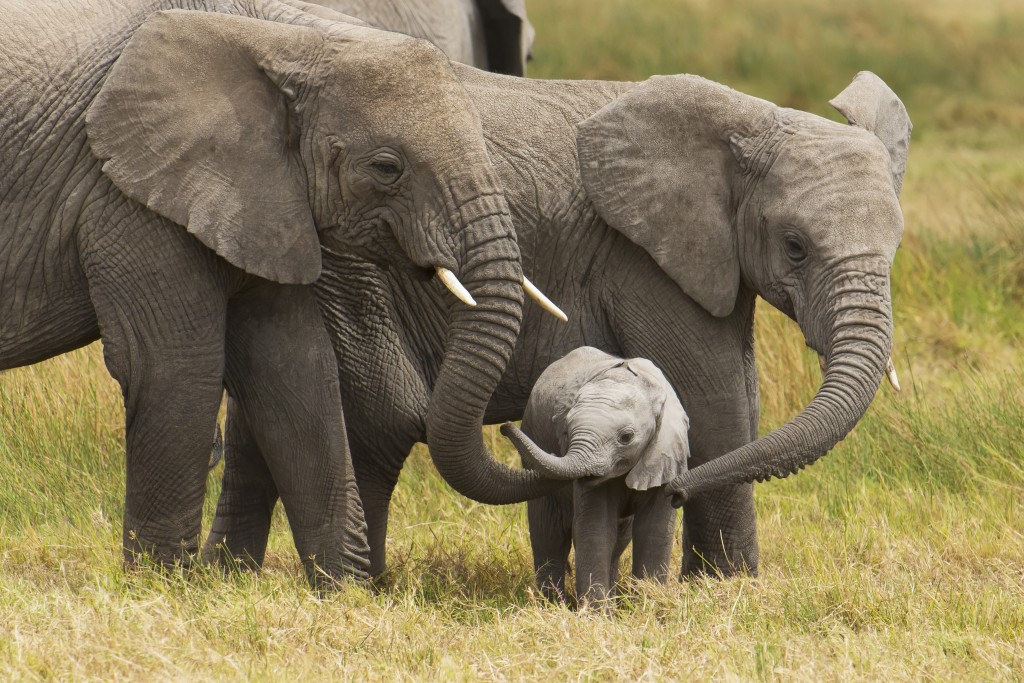
\includegraphics[width=0.9\textwidth]{figures/elephant.jpg}
			\end{center}
		\end{column}
		
		\begin{column}{0.5\textwidth}
			\begin{itemize}
				\item Begins breeding when 30
				\medskip
				\item Stops reproducing at 90
				\medskip
				\item Produces 6 offspring in these 6 years\\
				\bigskip
			\end{itemize}
			
			\begin{center}
				After 750 years, would be $\sim$19 million elephants descended \textcolor{red}{from a single pair}!
			\end{center}
		\end{column}
	\end{columns}
\end{frame}


%---------------------------%
% Natural Selection V       %
%---------------------------%
\begin{frame}[t]
\frametitle{Natural Selection}
\vspace{0.5cm}

	\begin{columns}
		\begin{column}{0.7\textwidth}
			\begin{enumerate}
				\item \textcolor{gray}{Individuals produce more offspring than the environment can support}
				\medskip
				\item Offspring vary in their ability to survive and reproduce
				\begin{center}
					\rule{0.5\textwidth}{0.5pt}\\
				\end{center}
				\smallskip
				\item \textcolor{gray}{Those individuals with variations that increase their ability to survive and reproduce will produce more offspring}
				\medskip
				\item \textcolor{gray}{These traits will be more prevalent in the next generation}
			\end{enumerate}
		\end{column}
		
		\begin{column}{0.3\textwidth}
			\begin{center}
				\includegraphics[width=0.9\textwidth]{figures/Darwin.jpg}
			\end{center}
		\end{column}
	\end{columns}
\end{frame}


%---------------------------%
% Natural Selection VI      %
%---------------------------%
\begin{frame}[t]
\frametitle{Natural Selection}
\vspace{0.5cm}

	\begin{columns}
		\begin{column}{0.7\textwidth}
			\begin{center}
				
\includegraphics[width=0.9\textwidth]{figures/individuality.jpg}
			\end{center}
		\end{column}
		
		\begin{column}{0.3\textwidth}
			\begin{center}
				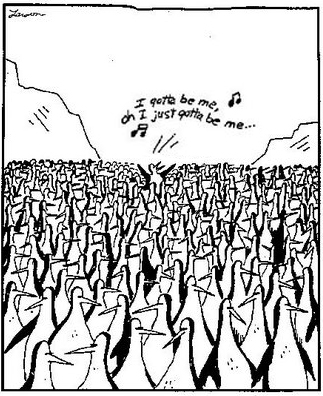
\includegraphics[width=0.9\textwidth]{figures/penguin.jpg}
			\end{center}
		\end{column}
	\end{columns}
\end{frame}


%---------------------------%
% Natural Selection VII     %
%---------------------------%
\begin{frame}[t]
\frametitle{Natural Selection}
\vspace{0.5cm}

	\begin{columns}
		\begin{column}{0.7\textwidth}
			\begin{enumerate}
				\item Individuals produce more offspring than the environment can support
				\medskip
				\item Offspring vary in their ability to survive and reproduce
				\begin{center}
					\rule{0.5\textwidth}{0.5pt}\\
				\end{center}
				\smallskip
				\item Those individuals with variations that increase their ability to survive and reproduce will produce more offspring
				\medskip
				\item These traits will be more prevalent in the next generation
			\end{enumerate}
		\end{column}
		
		\begin{column}{0.3\textwidth}
			\begin{center}
				\includegraphics[width=0.9\textwidth]{figures/Darwin.jpg}
			\end{center}
		\end{column}
	\end{columns}
\end{frame}


%---------------------------%
%  Fitness I                %
%---------------------------%
\begin{frame}[t]
\frametitle{Fitness}
\vspace{0.25cm}
	``Fitness'' refers to the number of offspring (or really the \# of genes) an individual contributes to future generations\\
	
	\vspace{1.0cm}
	
	``Survival of the fittest'' is not an accurate description of evolution\\
		\smallskip
		\begin{itemize}
			\item Survival means nothing (in evolutionary terms) except for how it influences reproductive success
		\end{itemize}
\end{frame}


%---------------------------%
%  Fitness II               %
%---------------------------%
\begin{frame}[t]
\frametitle{Two men}
\vspace{0.25cm}

	\begin{columns}[t]
		\begin{column}{0.5\textwidth}
			\begin{center}
				Man ``A'' is athletic, healthy, lived to be 109, had 2 kids and 4 grandkids\\
				\vspace{0.5cm}
				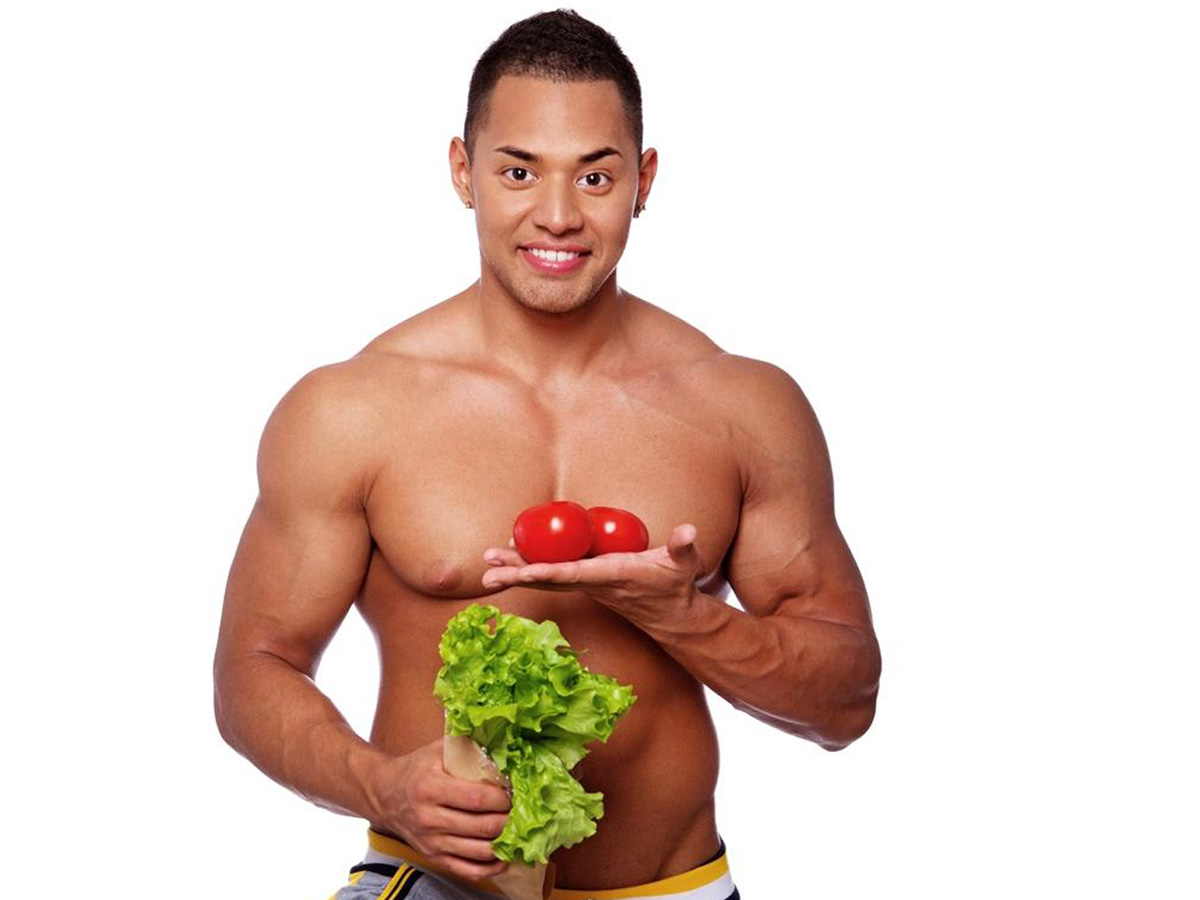
\includegraphics[width=0.7\textwidth]{figures/healthy.jpg}
			\end{center}
		\end{column}
		
		\begin{column}{0.5\textwidth}
			\begin{center}
				Man ``B'' is lazy, unhealthy, died at 50, had 4 kids and 8 grandkids\\
				\vspace{0.5cm}
				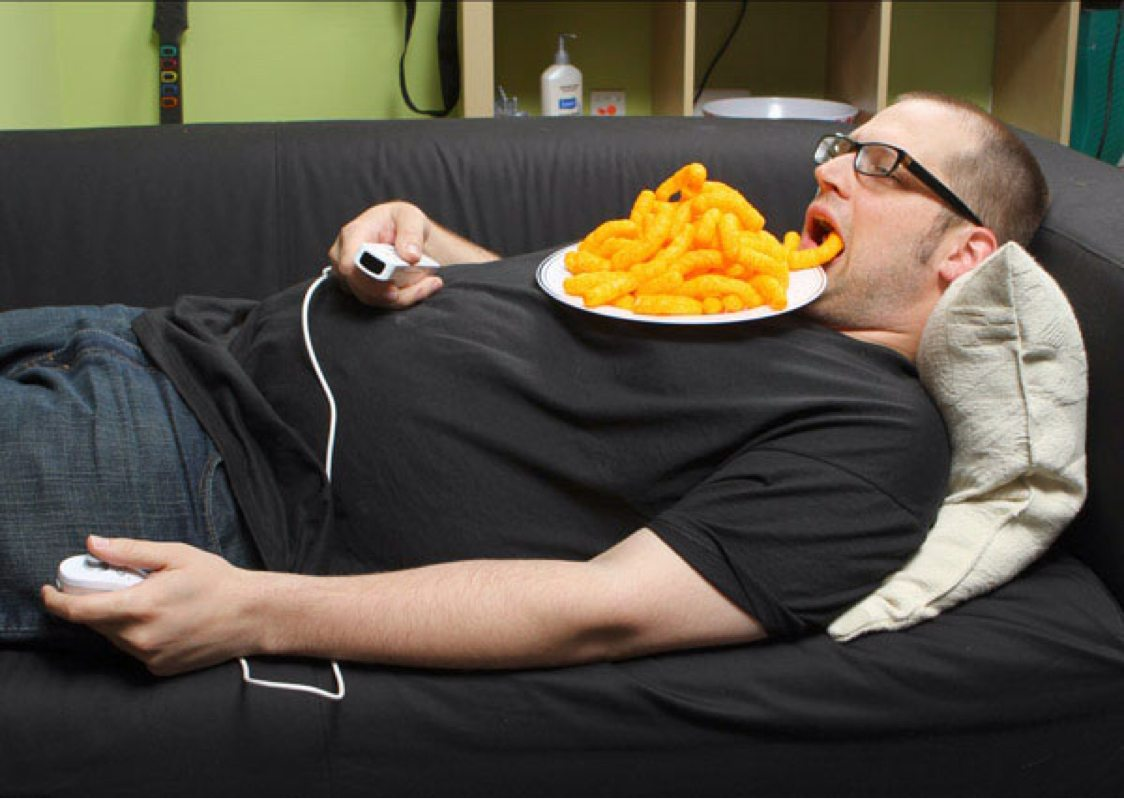
\includegraphics[width=0.7\textwidth]{figures/lazy.jpg}
			\end{center}
		\end{column}
	\end{columns}
	
	\vspace{0.5cm}
	
	\begin{center}
		\textcolor{myblue}{Who has higher evolutionary fitness?}
	\end{center}
\end{frame}


%---------------------------%
%     Mice                 %
%---------------------------%
\begin{frame}
\frametitle{Pocketmouse Example}

	\begin{center}
		\href{https://www.youtube.com/watch?v=sjeSEngKGrg}{\LARGE{VIDEO}}
	\end{center}
\end{frame}


%--------------------%
% Questions          %
%--------------------%
\begin{frame}
	\begin{center}
		\textcolor{myblue}{\LARGE{Questions?}}
	\end{center}	
\end{frame}    


%---------------------------%
%     Spiders               %
%---------------------------%
\begin{frame}
\frametitle{Redback Spider}

	\begin{center}
		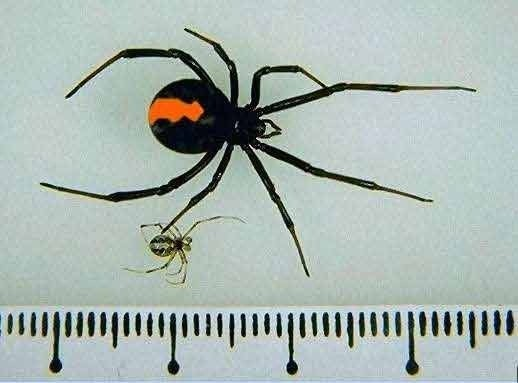
\includegraphics[width=0.4\textwidth]{figures/redback1.jpg}\\
		
		\vspace{0.5cm}
		
		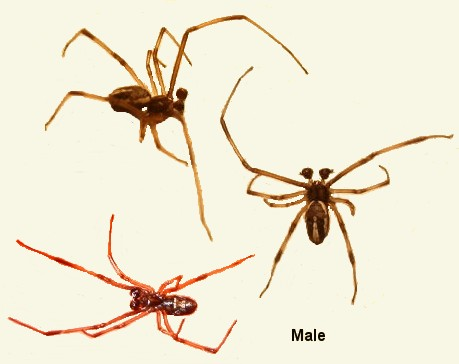
\includegraphics[width=0.4\textwidth]{figures/redback2.jpg}\\
	\end{center}
\end{frame}


%---------------------------%
%     Spiders               %
%---------------------------%
\begin{frame}[t]
\frametitle{Redback Spider}
\vspace{0.5cm}

	For this to have evolved, what predictions can you make about the biology of these spiders?
\end{frame}


%---------------------------%
% Misconceptions I          %
%---------------------------%
\begin{frame}
	\begin{center}
		\textcolor{myblue}{\LARGE{Common Misconceptions}}
	\end{center}	
\end{frame}


%---------------------------%
% Misconceptions II         %
%---------------------------%
\begin{frame}[t]
\frametitle{Common Misconceptions}
\vspace{0.5cm}
	
	\textbf{\textcolor{myblue}{1.} Darwin was the first to propose evolution}
	
	\medskip
	
	\begin{itemize}
		\item Start with the ``fixity of species''
		\medskip
		\item Many others thought this wasn't so, and thought that organisms evolve
	\end{itemize}
\end{frame}


%---------------------------%
% Misconceptions III        %
%---------------------------%
\begin{frame}[t]
\frametitle{Comte de Buffon (1707--1788)}
\framesubtitle{French naturalist}
	
	\begin{center}
		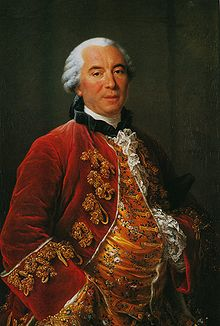
\includegraphics[width=0.20\textwidth]{figures/buffon.jpg}\\
	\end{center}
	
	\vspace{0.25cm}
	
	\begin{itemize}
		\item Despite similar environments, different regions had distinct organisms (biogeography)
		\medskip
		\item Species both ``improved'' and ``degenerated'' after dispersing from a centre of creation
	\end{itemize}
\end{frame}


%---------------------------%
% Misconceptions IV         %
%---------------------------%
\begin{frame}[t]
\frametitle{Erasmus Darwin (1731--1802)}
	
	\begin{center}
		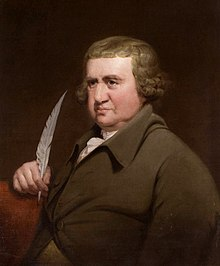
\includegraphics[width=0.20\textwidth]{figures/edarwin.jpg}\\
	\end{center}
	
	\vspace{0.25cm}
	
	\begin{itemize}
		\item ``All warm-blooded animals have arisen from one living filament'' (1796) 
		\medskip
		\item In 1802, describes the rise of life from minute organisms living in the mud to all of its modern diversity
	\end{itemize}
\end{frame}


%---------------------------%
% Misconceptions V          %
%---------------------------%
\begin{frame}[t]
\frametitle{Jean-Baptiste Lamarck (1744--1829)}
	
	\begin{columns}
		\begin{column}{0.5\textwidth}
			\begin{center}
				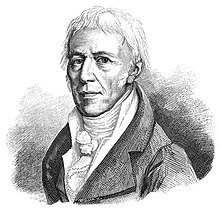
\includegraphics[width=0.50\textwidth]{figures/lamarck.jpg}
			\end{center}
		\end{column}
		
		\begin{column}{0.5\textwidth}
			\begin{center}
				First comprehensive theory of evolution$\ldots$now known to be incorrect
			\end{center}
		\end{column}	
	\end{columns}
	
	\vspace{0.5cm}
	
	\begin{itemize}
		\item All species (including humans) are derived from the gradual evolution of other species 
		\medskip
		\item Occurred through the inheritance of acquired traits
		\medskip
		\item All organisms progress from simple to complex forms
	\end{itemize}
	
	\begin{tikzpicture}[overlay]
		\node at (11, 2.5) (node1) {
\includegraphics[width=0.05\textwidth]{figures/happy.png}};
		\node at (11, 1.5) (node2) {
\includegraphics[width=0.05\textwidth]{figures/frown.png}};
		\node at (11, 0.7) (node3) {
\includegraphics[width=0.05\textwidth]{figures/frown.png}};
	\end{tikzpicture}
\end{frame}


%---------------------------%
% Misconceptions VI         %
%---------------------------%
\begin{frame}[t]
\frametitle{What Did Darwin Do That Was So Important?}
	
	\begin{center}
		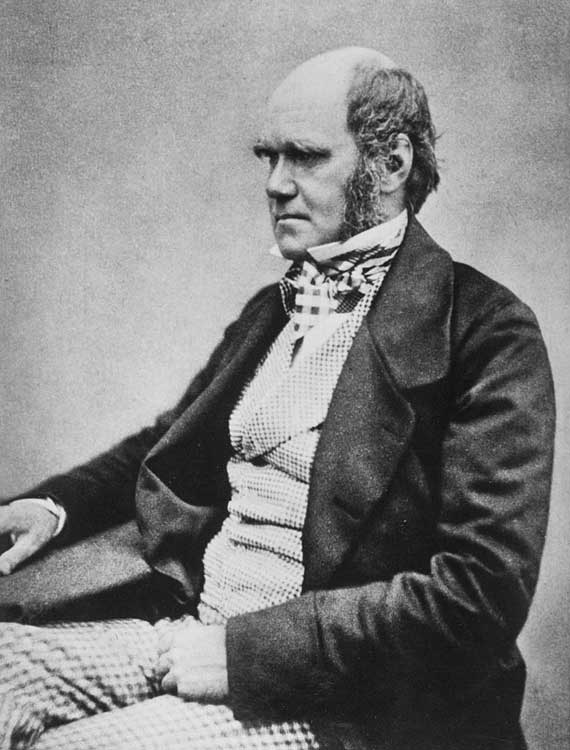
\includegraphics[width=0.20\textwidth]{figures/darwin.jpg}\\
	\end{center}
	
	\vspace{0.25cm}
	
	\begin{itemize}
		\item Published the most extensive and convincing evidence/argument for evolution - convinced the scientific community (1859) 
		\medskip
		\item Developed the first (and arguably most important) accurate mechanism---\textcolor{myblue}{natural selection}
	\end{itemize}
\end{frame}


%---------------------------%
% Misconceptions VII        %
%---------------------------%
\begin{frame}[t]
\frametitle{Common Misconceptions}
\vspace{0.5cm}
	
	\textbf{\textcolor{gray}{1. Darwin was the first to propose evolution}}\\
	\medskip
	\textbf{\textcolor{myblue}{2.} Evolution is ``only'' a theory}
\end{frame}


%---------------------------%
% Misconceptions VIII       %
%---------------------------%
\begin{frame}[t]
\frametitle{Common Misconceptions}
\vspace{0.5cm}
	
	\textbf{\textcolor{gray}{1. Darwin was the first to propose evolution}}\\
	\medskip
	\textbf{\textcolor{gray}{2. Evolution is ``only'' a theory}}\\
	\medskip
	\textbf{\textcolor{myblue}{3.} Evolution is progressive, moving towards some ultimate ``goal''}
\end{frame}


%---------------------------%
% Misconceptions IX         %
%---------------------------%
\begin{frame}[t]
\frametitle{Common Misconceptions}
\vspace{0.5cm}

	Natural selection is just the differential fitness of individuals in the \textcolor{red}{\emph{current environment}}!\\
	\bigskip
	
	\begin{itemize}
		\item No foresight
		\medskip
		\item What is ``best'' will depend on specific environment (which will change over time!)
		\medskip
		\item Each stage must provide an advantage
	\end{itemize}	
\end{frame}


%---------------------------%
% Misconceptions  X         %
%---------------------------%
\begin{frame}[t]
\frametitle{Common Misconceptions}

	\begin{tikzpicture}[overlay]
		\node at (5, -2) (node1) {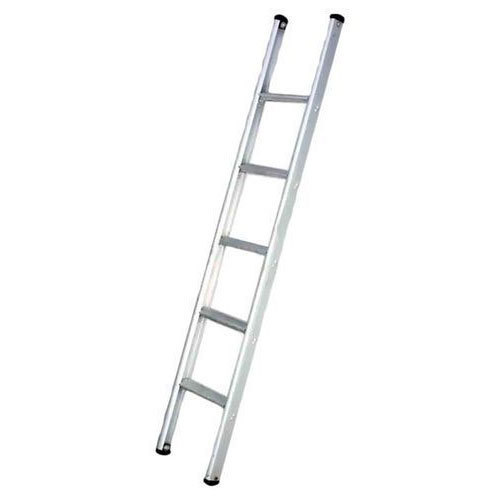
\includegraphics[width=0.3\textwidth]{figures/ladder.jpeg}};
		\node at (2.5, -0.3) (humans) {Humans};
		\node at (2.5, -1.3) (mammals) {Mammals};
		\node at (2.5, -2.3) (insects) {Insects};
		\node at (2.5, -3.3) (slime) {Slimy things};
		\node at (7.5, -0.3) (more) {\textcolor{myblue}{``More evolved''}};
		\node at (7.5, -3.3) (more) {\textcolor{myblue}{``Less evolved''}};
	\end{tikzpicture}
\end{frame}


%---------------------------%
% Misconceptions  XI        %
%---------------------------%
\begin{frame}[t]
\frametitle{Common Misconceptions}

	\begin{tikzpicture}[overlay]
		\node at (5, -2) (node1) {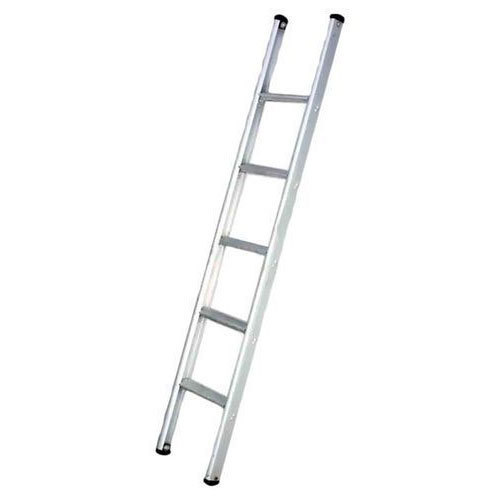
\includegraphics[width=0.3\textwidth]{figures/ladder.jpeg}};
		\node at (2.5, -0.3) (humans) {Humans};
		\node at (2.5, -1.3) (mammals) {Mammals};
		\node at (2.5, -2.3) (insects) {Insects};
		\node at (2.5, -3.3) (slime) {Slimy things};
		\node at (7.5, -0.3) (more) {\textcolor{myblue}{``More evolved''}};
		\node at (7.5, -3.3) (more) {\textcolor{myblue}{``Less evolved''}};
		\node at (5, -2) (no) {
\includegraphics[width=0.3\textwidth]{figures/no.png}};
		\node at (5, -5) (text){\textcolor{red}{Cannot refer to ``higher'' and ``lower'' organisms}};
	\end{tikzpicture}
\end{frame}


%---------------------------%
% Misconceptions  XII       %
%---------------------------%
\begin{frame}[t]
\frametitle{Common Misconceptions}
\vspace{0.5cm}
	
	\textbf{\textcolor{gray}{1. Darwin was the first to propose evolution}}\\
	\medskip
	\textbf{\textcolor{gray}{2. Evolution is ``only'' a theory}}\\
	\medskip
	\textbf{\textcolor{gray}{3. Evolution is progressive, moving towards some ultimate ``goal''}}\\
	\medskip
	\textbf{\textcolor{myblue}{4.} Contemporary species evolved from other contemporary species}\\
		
		\medskip
		
		\begin{itemize}
			\item ``Humans evolved from chimpanzees''
		\end{itemize}
\end{frame}


%---------------------------%
% Misconceptions  XIII      %
%---------------------------%
\begin{frame}[t]
\frametitle{Common Misconceptions}
\vspace{0.5cm}
	
	\begin{center}
		\textcolor{myblue}{Contemporary species share a common ancestor!}\\
		
		\vspace{0.75cm}
		
		\includegraphics[width=0.7\textwidth]{figures/ape.png}
	\end{center}
\end{frame}


%---------------------------%
% Misconceptions  XIV       %
%---------------------------%
\begin{frame}[t]
\frametitle{Common Misconceptions}
\vspace{0.5cm}
	
	\begin{center}
		\includegraphics[width=0.7\textwidth]{figures/ape2.jpg}
	\end{center}
\end{frame}


%---------------------------%
% Misconceptions  XV       %
%---------------------------%
\begin{frame}[t]
\frametitle{Common Misconceptions}
\vspace{0.5cm}
	
	\begin{center}
		\includegraphics[width=0.7\textwidth]{figures/ape2.jpg}
	\end{center}
	
	\begin{tikzpicture}[overlay]
		\node at (5, 1.8) (no) {\includegraphics[width=0.3\textwidth]{figures/no.png}};
	\end{tikzpicture}
\end{frame}


%--------------------%
% Questions          %
%--------------------%
\begin{frame}
	\begin{center}
		\textcolor{myblue}{\LARGE{Questions?}}
	\end{center}	
\end{frame}       


%---------------------------%
% Proximate vs Ultimate     %
%---------------------------%
\begin{frame}[t]
\frametitle{How We Approach Biological Questions}
\vspace{0.5cm}
	
	\begin{block}{Proximate Causation}
		\textbf{How} something works/occurs (mechanistic).\\
		\medskip
		\emph{How is this gene turned on or off?\\
		How do individuals of this species choose a mate?} 
	\end{block}
	
	\vspace{0.5cm}

	\begin{block}{Ultimate Causation}
		\textbf{Why} something works/occurs the way it does (evolutionary). \\
		\medskip
		\emph{Why has this process evolved for the regulation of this gene?\\
		Why have these mechanisms evolved by which these individuals select mates?}
	\end{block}
\end{frame}


%--------------------%
% Boardwork          %
%--------------------%
\begin{frame}
	\begin{center}
		\textcolor{myblue}{\LARGE{Board Work?}}
	\end{center}	
\end{frame}  


%--------------------%
% Beagle             %
%--------------------%
\begin{frame}
	\begin{columns}
		\begin{column}{0.5\textwidth}
			\begin{center}
				\includegraphics[width=0.8\textwidth]{figures/beagle.png}
			\end{center}
		\end{column}
		
		\begin{column}{0.5\textwidth}
			\begin{center}
				\includegraphics[width=1.0\textwidth]{figures/voyage.jpg}
			\end{center}
		\end{column}
	\end{columns}
\end{frame}  


%--------------------%
% Lyell              %
%--------------------%
\begin{frame}
	\begin{columns}
		\begin{column}{0.5\textwidth}
			\begin{center}
				\includegraphics[width=0.8\textwidth]{figures/Lyell.jpg}
			\end{center}
		\end{column}
		
		\begin{column}{0.5\textwidth}
			\begin{center}
				\includegraphics[width=1.0\textwidth]{figures/lyell-principles.jpg}
			\end{center}
		\end{column}
	\end{columns}
\end{frame}  


%--------------------%
% Islands            %
%--------------------%
\begin{frame}
	\begin{columns}
		\begin{column}{0.5\textwidth}
			\begin{center}
				\includegraphics[width=0.8\textwidth]{figures/mockingbirds.png}
			\end{center}
		\end{column}
		
		\begin{column}{0.5\textwidth}
			\begin{center}
				\includegraphics[width=1.0\textwidth]{figures/tortoises.jpg}
			\end{center}
		\end{column}
	\end{columns}
\end{frame}  


%----------------------%
% Artificial Selection %
%----------------------%
\begin{frame}
	\begin{columns}
		\begin{column}{0.5\textwidth}
			\begin{center}
				\includegraphics[width=1.0\textwidth]{figures/dogs.jpg}
			\end{center}
		\end{column}
		
		\begin{column}{0.5\textwidth}
			\begin{center}
				\includegraphics[width=1.0\textwidth]{figures/mustard.jpg}
			\end{center}
		\end{column}
	\end{columns}
\end{frame} 


%----------------------%
% Natural Selection    %
%----------------------%
\begin{frame}
	\begin{columns}
		\begin{column}{0.5\textwidth}
			\begin{center}
				\includegraphics[width=0.6\textwidth]{figures/darwintree.jpg}
			\end{center}
		\end{column}
		
		\begin{column}{0.5\textwidth}
			\begin{center}
				\includegraphics[width=1.0\textwidth]{figures/darwintree2.jpg}
			\end{center}
		\end{column}
	\end{columns}
\end{frame}  


%----------------------%
% Reading              %
%----------------------%
\begin{frame}
	\begin{columns}
		\begin{column}{0.5\textwidth}
			\begin{center}
				\includegraphics[width=0.45\textwidth]{figures/book1.jpg}\\
				\vspace{0.25cm}
				\includegraphics[width=0.45\textwidth]{figures/book2.jpg}
			\end{center}
		\end{column}
		
		\begin{column}{0.5\textwidth}
			\begin{center}
				\includegraphics[width=0.45\textwidth]{figures/book3.jpg}\\
				\vspace{0.25cm}
				\includegraphics[width=0.45\textwidth]{figures/book4.jpg}
			\end{center}
		\end{column}
	\end{columns}
\end{frame}  


%----------------------%
% Wallace              %
%----------------------%
\begin{frame}
	\begin{columns}
		\begin{column}{0.5\textwidth}
			\begin{center}
				\includegraphics[width=0.5\textwidth]{figures/wallace1.jpg}
			\end{center}
		\end{column}
		
		\begin{column}{0.5\textwidth}
			\begin{center}
				\includegraphics[width=0.8\textwidth]{figures/wallace2.jpg}
			\end{center}
		\end{column}
	\end{columns}
\end{frame}  


%----------------------%
% Wallace              %
%----------------------%
\begin{frame}
	\begin{columns}
		\begin{column}{0.5\textwidth}
			\begin{center}
				\includegraphics[width=0.8\textwidth]{figures/wallaces-line.jpg}
			\end{center}
		\end{column}
		
		\begin{column}{0.5\textwidth}
			\begin{center}
				\includegraphics[width=0.8\textwidth]{figures/wallaces-line2.png}
			\end{center}
		\end{column}
	\end{columns}
\end{frame}  


\end{document}